% !TeX spellcheck = es_ES
%----------------------------------------------------------------------------------------
%	PACKAGES AND OTHER DOCUMENT CONFIGURATIONS
%----------------------------------------------------------------------------------------

\documentclass[fleqn,10pt]{SelfArx} % Document font size and equations flushed left
%\usepackage{chemmacros}
\usepackage{ifthen}
\usepackage{calc}
\usepackage{microtype}
\usepackage{ifpdf}
\usepackage[utf8]{inputenc}
\usepackage{amsmath, amsfonts, amssymb}
\usepackage{graphicx, xcolor}
\usepackage{booktabs}
\usepackage{fancyhdr}
\usepackage{lastpage}
\usepackage{titlesec}
\usepackage{titletoc}
\usepackage{enumitem}
%\usepackage{cuted}
\usepackage[version=3]{mhchem}
\usepackage{graphbox}
\usepackage{tabularx}
\usepackage{multirow}
%----------------------------------------------------------------------------------------
%	COLUMNS
%----------------------------------------------------------------------------------------

\setlength{\columnsep}{0.55cm} % Distance between the two columns of text
\setlength{\fboxrule}{1pt} % Width of the border around the abstract

%----------------------------------------------------------------------------------------
%	COLORS
%----------------------------------------------------------------------------------------

\definecolor{color1}{RGB}{0,94,157} % Color of the article title and sections
\definecolor{color2}{RGB}{255,243,210} % Color of the boxes behind the abstract and headings

%----------------------------------------------------------------------------------------
%	HYPERLINKS
%----------------------------------------------------------------------------------------

\usepackage{hyperref} % Required for hyperlinks
\hypersetup{hidelinks,colorlinks,breaklinks=true,urlcolor=color2,citecolor=color1,linkcolor=color1,bookmarksopen=false,pdftitle={Title},pdfauthor={Author}}

%----------------------------------------------------------------------------------------
%	ARTICLE INFORMATION
%----------------------------------------------------------------------------------------

\JournalInfo{L. de Qu\'imica inorg\'anica II, No. 5, 2016-20} % Journal information
%\Archive{Additional note} % Additional notes (e.g. copyright, DOI, review/research article)

\PaperTitle{Determinaci\'on de la energ\'ia de estabilizaci\'on} % Article title

\Authors{Juan Barbosa{\color{color1}\textsuperscript{1}\textsuperscript{,2}*},
	Alejandro Camacho{\color{color1}\textsuperscript{1}\textsuperscript{,3}**}} %
%Authors
\affiliation{{\color{color1}\textsuperscript{1}}\textit{Departamento de Qu\'imica, Universidad de los Andes, Bogot\'a, Colombia}} % Author affiliation
\affiliation{{\color{color1}\textsuperscript{2}}\textit{Departamento de F\'isica, Universidad de los Andes, Bogot\'a, Colombia}} % Author affiliation
\affiliation{{\color{color1}\textsuperscript{3}}\textit{Departamento de	F\'isica, Universidad Nacional, Bogot\'a, Colombia}}
\affiliation{{\color{color1}*}\textbf{Email}: js.barbosa10@uniandes.edu.co} %
%Corresponding author
\affiliation{{\color{color1}**}\textbf{Email}: a.camacho10@uniandes.edu.co}
\Keywords{Tanabe - Sugano, campo cristalino, campo de ligandos, serie espectroqu\'imica, energ\'ia de estabilizaci\'on} %
%Keywords - if you don't want any simply remove all the text between the curly
%brackets
\newcommand{\keywordname}{Keywords} % Defines the keywords heading name

%----------------------------------------------------------------------------------------
%	ABSTRACT
%----------------------------------------------------------------------------------------
\Abstract
{
	El complejo tris(etilendiamin)cromo (III) es sintetizado en el laboratorio. Las energ\'ias de estabilizaci\'on de los compuestos tris(etilendiamin)cromo (III) y tetra(acuo)di(cloro)cromo (III) se determinan en $\Delta_0 = 2.63$ ,  $\Delta_0 = 1.98$ eV correspondientemente. Adicionalmente se realizan estudios te\'oricos entorno al acetilacetonato de cromo (III), los resultados son comparados con los valores te\'oricos asociados al diagrama de Tanabe - Sugano para un metal de transici\'on d$^3$.
}
%----------------------------------------------------------------------------------------

\begin{document}
	\flushbottom % Makes all text pages the same height
	\maketitle % Print the title and abstract box
	%\tableofcontents % Print the contents section
	\thispagestyle{empty} % Removes page numbering from the first page
	%----------------------------------------------------------------------------------------
	%	ARTICLE CONTENTS
	%----------------------------------------------------------------------------------------
	\section*{Introducci\'on}
	Si bien los complejos de coordinaci\'on eran sintetizados con frecuencia antes del siglo XVIII dado su atractivo color para los pint\'ores y la industria textil de la \'epoca, fue \'unicamente hasta el siglo XIX con la teor\'ia de Werner que el estudio de formal de los compuestos de coordinaci\'on tuvo un inicio. La teor\'ia de Werner fue la primera en considerar esp\'ecies neutras ligadas a un metal. Si bien la teor\'ia de Werner logr\'o explicar la estequiometr\'ia de los complejos de coordinaci\'on y su estructura, adem\'as de la distinci\'on entre la valencia primaria y secundaria, t\'erminos hoy conocidos como estado de oxidaci\'on y n\'umero de coordinaci\'on, la teor\'ia no daba explicaci\'on sobre la naturaleza del enlace \cite{Orbitals}.
	
	\begin{figure}[h]
		\centering
		\begin{tabular}{cc}
			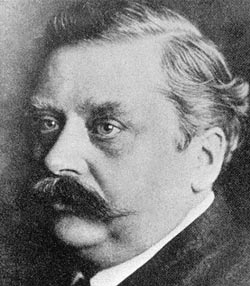
\includegraphics[width=0.5\linewidth]{images/werner.jpg}
			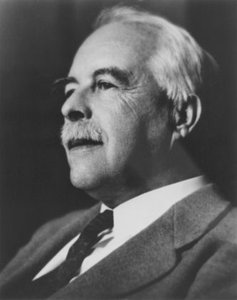
\includegraphics[width=0.452\linewidth]{images/lewis.jpg}
		\end{tabular}
		\caption{Alfred Werner \cite{Werner} y Gilbert Lewis \cite{Lewis}, grandes contribuyentes a la qu\'imica de coordinaci\'on.}
	\end{figure}
	
	El siguiente avance fue hecho por Gilbert N. Lewis, qu\'imico norteamericano, al generalizar el concepto de \'acido base extendiendolo hasta los complejos de coordinaci\'on, los cuales se originaban como aductos de la reacci\'on de una esp\'ecie que acepta electrones de otra que los cede, dichas esp\'ecies hoy reciben el nombre de \'acidos y bases de Lewis. Sobre el siglo XX surge la llamada teor\'ia del campo cristalino, la cual finalmente da explicaci\'on a la coloraci\'on de los complejos de coordinaci\'on, as\'i como las propiedades magn\'eticas del mismo. Con el desarrollo de la cu\'antica y la teor\'ia del orbital molecular, se incluyen mejoras a la teor\'ia del campo cristalino alcanzando as\'i la teor\'ia del campo de ligandos. En esta \'ultima teor\'ia se tienen en cuenta el caracter $\sigma$ \'o $\pi$ del enlace metal ligando, dando explicaci\'on la naturaleza del enlace coordinativo.
	
	Tanto en el campo cristalino como en el campo de ligandos, para un complejo octa\'edrico los orbitales $d$ se desdoblan debido a la geometr\'ia de los orbitales. En una geometr\'ia octa\'edrica los ligandos se ubican en los ejes $x$ y $y$ (ecuatoriales) y $z$ (axiales), en el caso de los orbitales $d_{z^2}$ y $d_{x^2-y^2}$ la energ\'ia aumentar\'a debido a que se encuentran en el eje de los ligandos como se observa en la \autoref{fig: orbitals}. Lo contrario sucede con los orbitales $d_{xy}$, $d_{xz}$ y $d_{yz}$ \cite{Orbitals}.
	\begin{figure}[h]
		\centering
		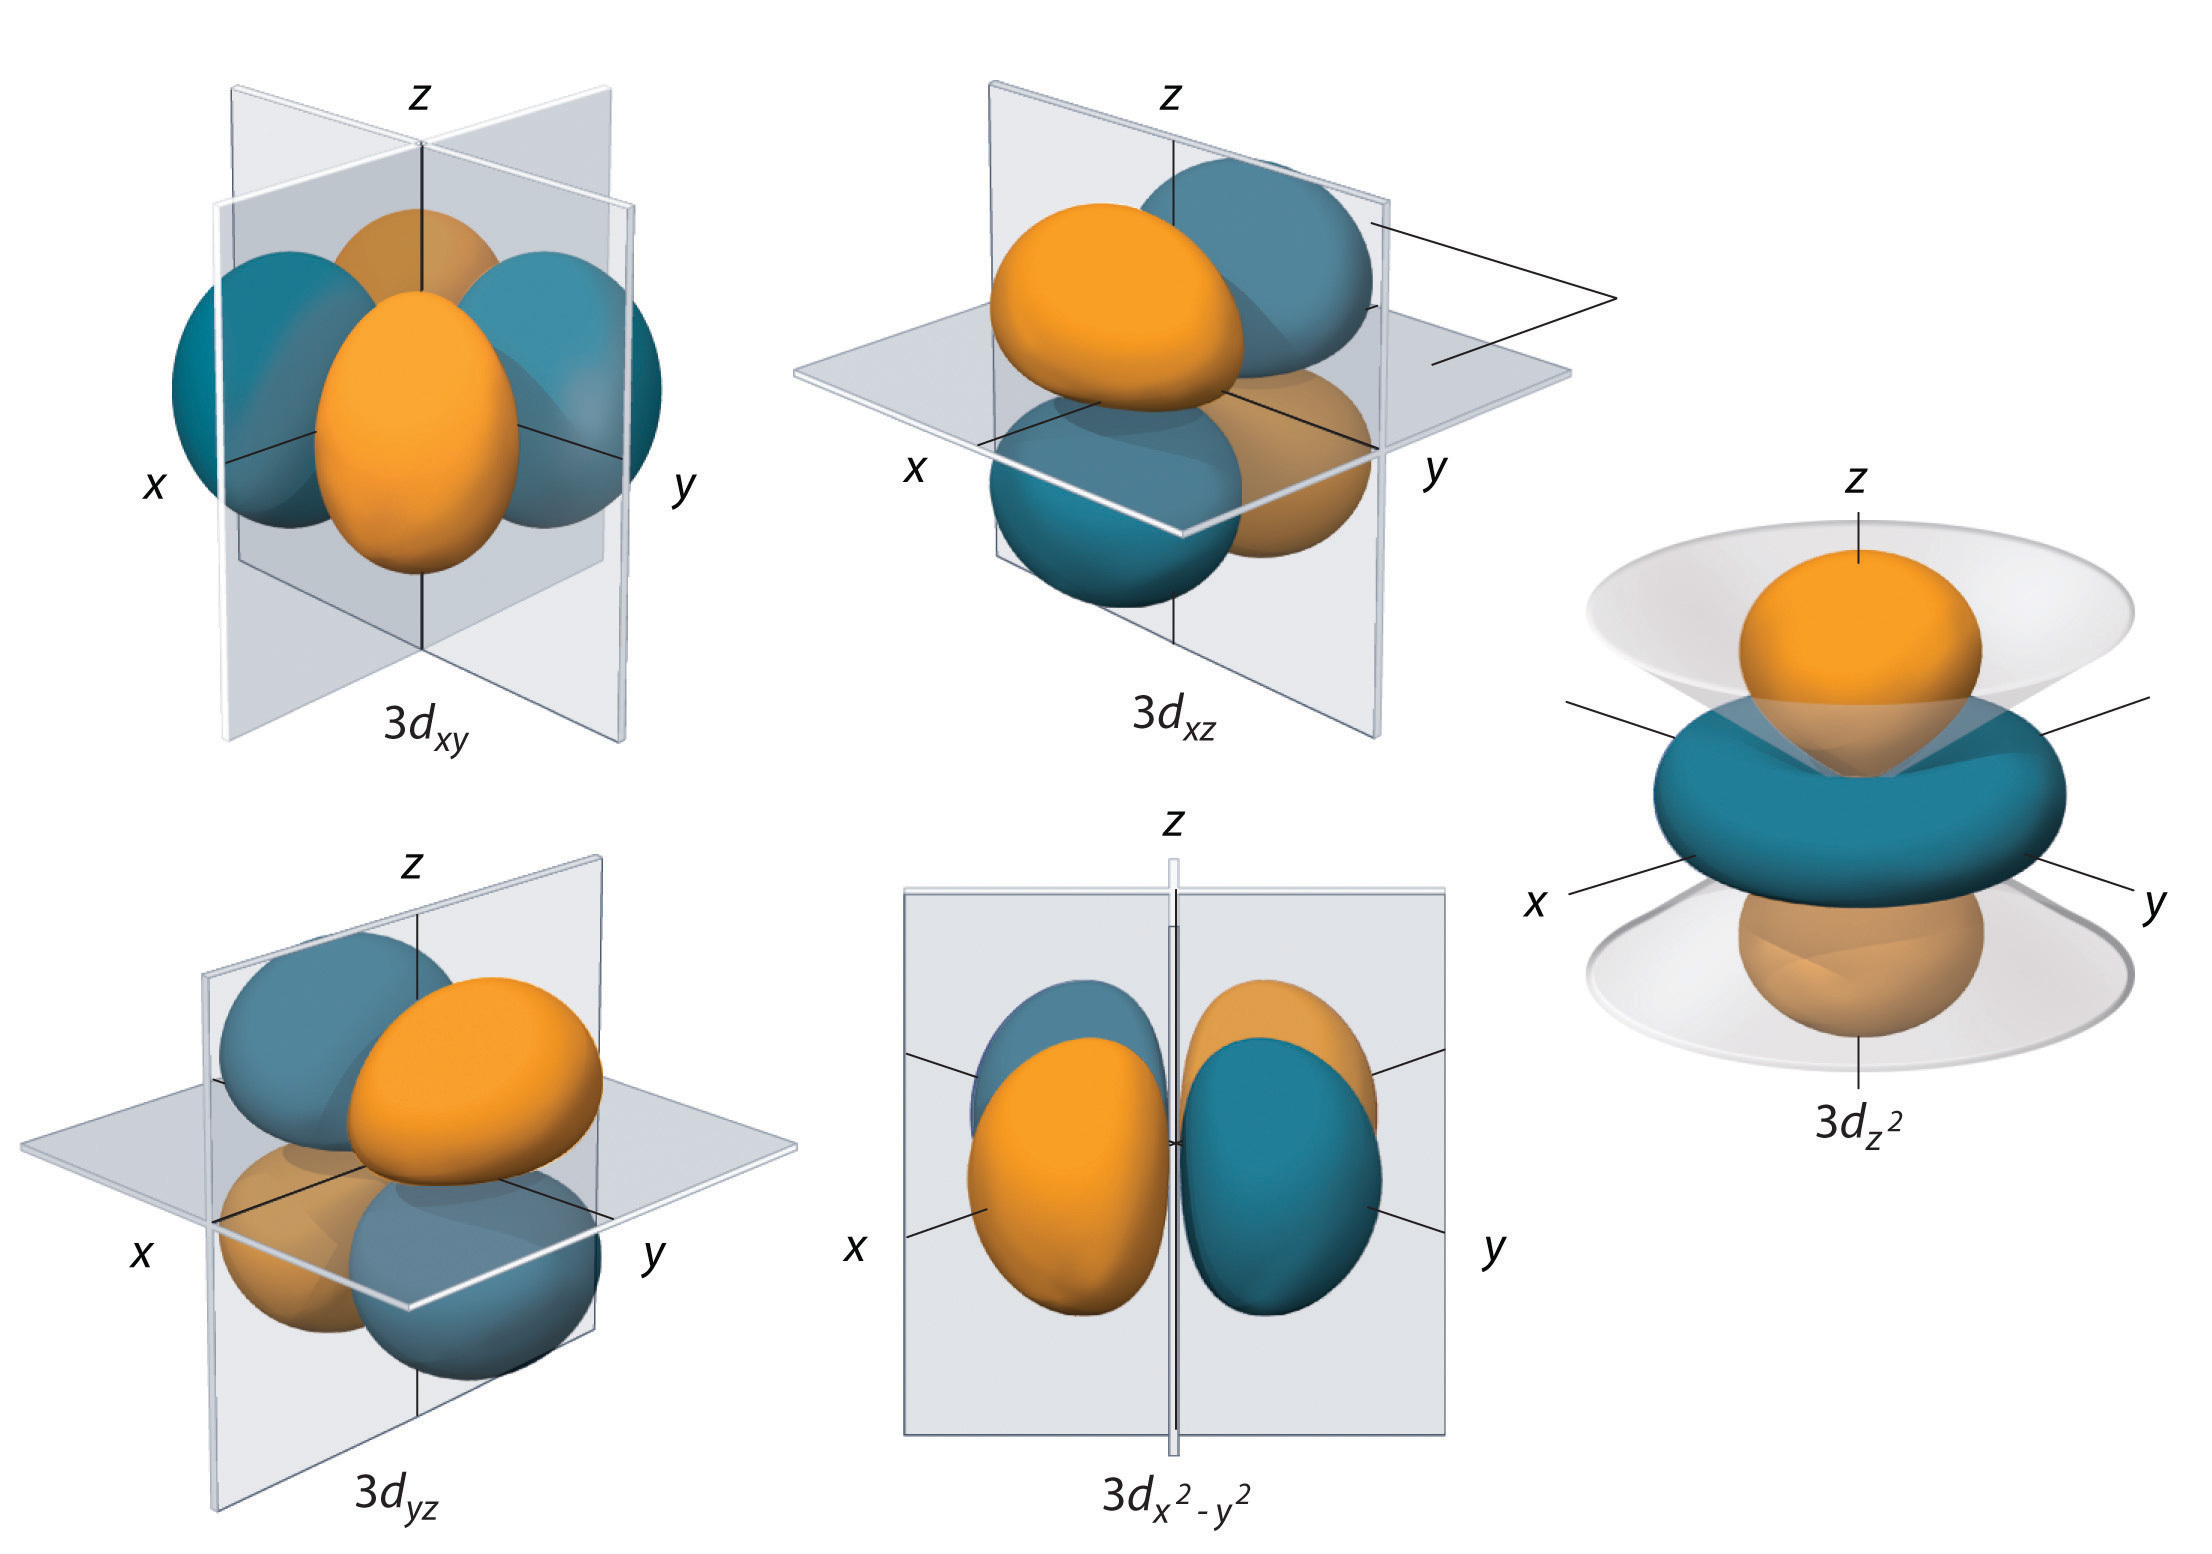
\includegraphics[width=0.8\linewidth]{images/orbitals.jpg}
		\caption{Geometr\'ia de los orbitales $d$ \cite{Orbitals}.}
		\label{fig: orbitals}
	\end{figure}
	\pagebreak
	
	La energ\'ia de desdoblamiento recibe el nombre de energ\'ia de estabilizaci\'on del campo y se simboliza como $\Delta_0$ como se observa en la \autoref{fig: splitting}. Adicionalmente es necesario tener en cuenta que debido a la simetr\'ia electr\'onica los orbitales $d_{z^2}$ y $d_{x^2-y^2}$ reciben el nombre de $e_g$ y se dice que est\'an doblemente degenerados. Los orbitales $d$ restantes reciben el nombre de $t_{2g}$ y se encuentran triplemente degenerados.
	\begin{figure}[h]
		\centering
		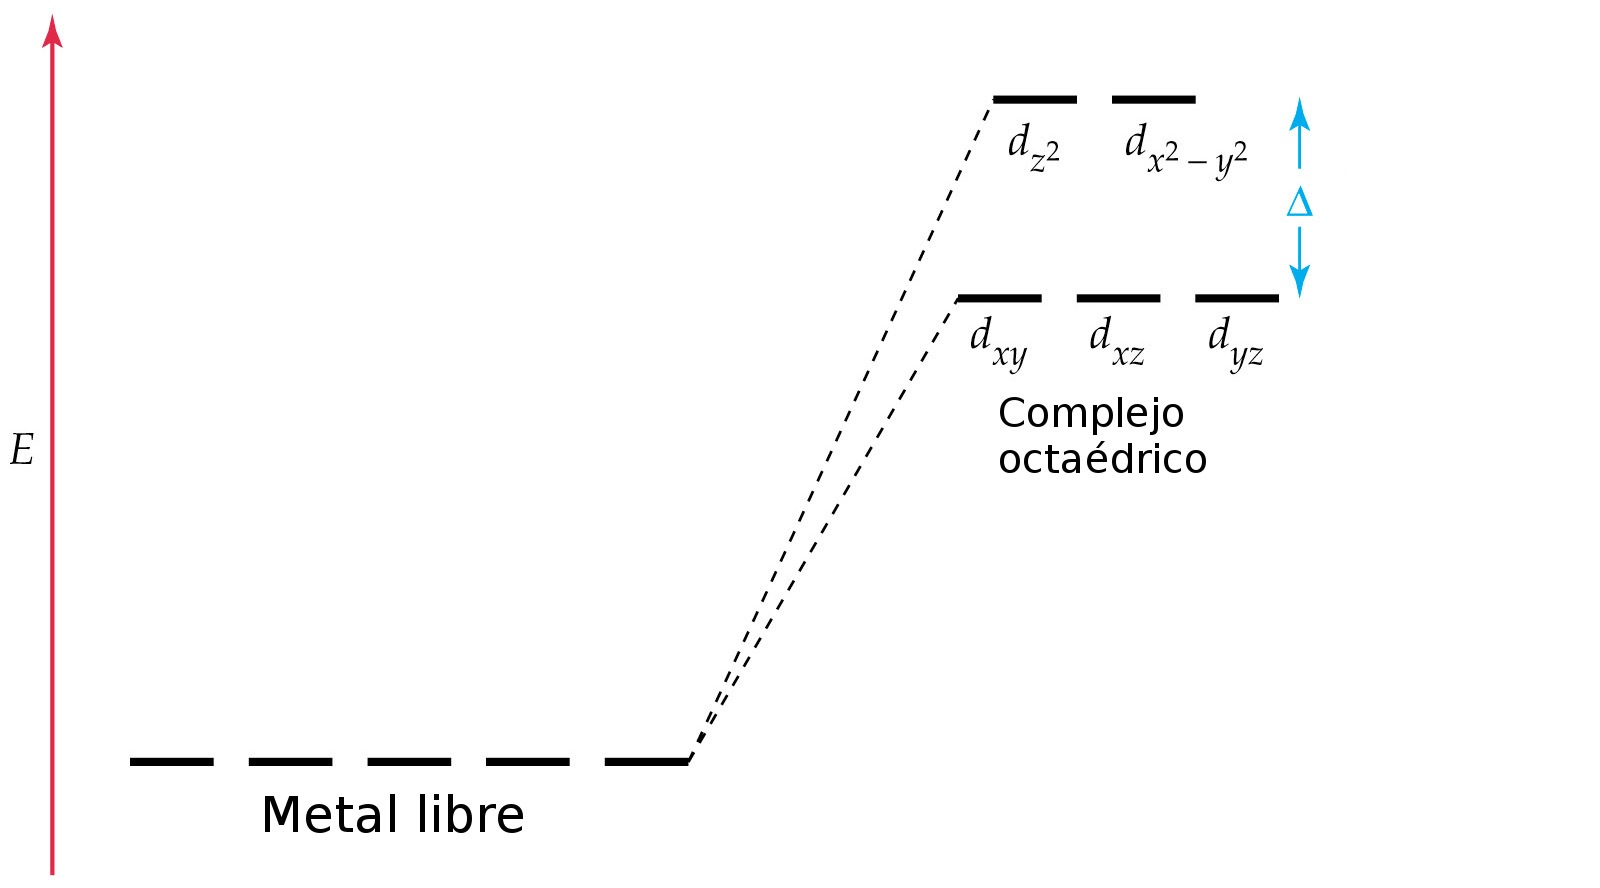
\includegraphics[width=\linewidth]{images/splitting.jpg}
		\caption{Desdoblamiento de los orbitales $d$ en un complejo octa\'edrico. Modificado de \cite{Orbitals}.}
		\label{fig: splitting}
	\end{figure}
	
	\section{Metodolog\'ia}
	En un beaker son adicionados 2 mL de \'acido clorh\'idrico 6 M junto con 1.0 g de z\'inc elemental. En un bal\'on de 50 mL son adicionados 2.632 g de \ce{CrCl3 . 6H2O} seguidos de 10 mL de etilendiamina pura y 10 mL de etanol, junto con el zinc previamente lavado con HCl. El bal\'on es sometido a reflujo sobre un ba\~no de arena por cerca de 90 minutos. El producto obtenido es filtrado al vac\'io y lavado continuamente con etanol fr\'io.
	\begin{figure}[h]
		\centering
		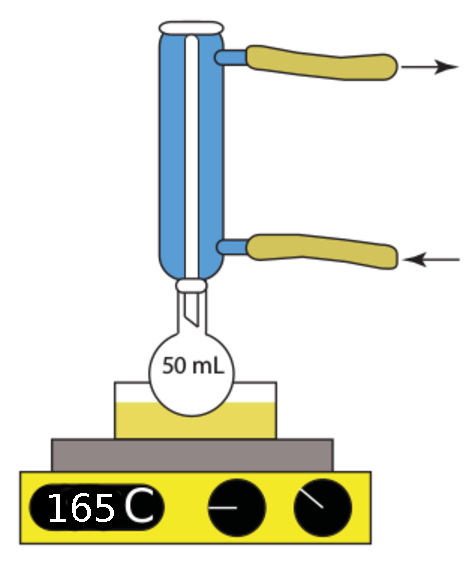
\includegraphics[width=0.6\linewidth]{images/Montaje.pdf}
		\caption{Montaje experimental usado en el laboratorio.}
	\end{figure}	
	\pagebreak
	
	\section{Resultados y Discusi\'on}	
	Los complejos sintetizados corresponden con el  \ce{[Cr(en)3]} y el \ce{[CrCl2(H2O)4]+}, los mismos fueron analizados por espectroscop\'ia UV-vis. Para ambos se obtuvieron dos bandas de absorci\'on caracter\'isticas, las concentraciones de diluci\'on fueron: 5.30 mM y 4.65 mM, para el \ce{[Cr(en)3]} y \ce{[CrCl2(H2O)4]+} correspondientemente.
	
	\begin{figure*}[h]
		\centering
		\begin{tabular}{cccc}
			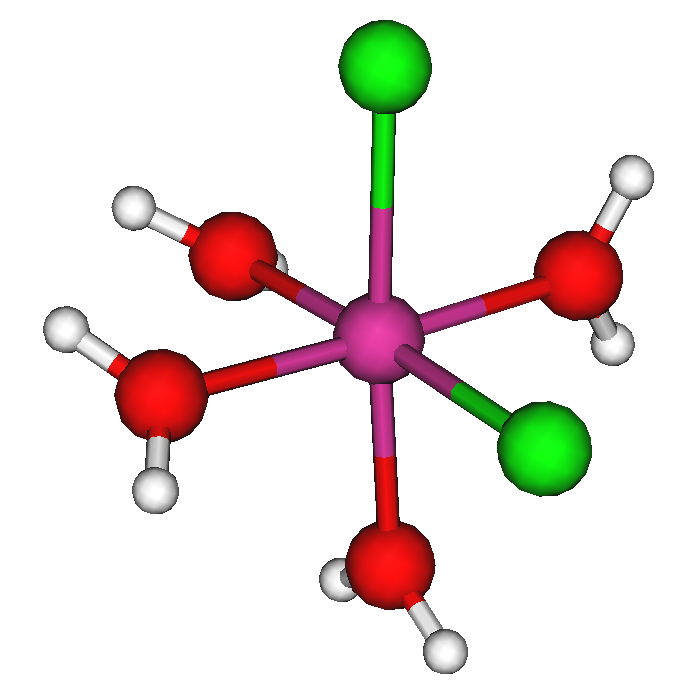
\includegraphics[width=0.2\linewidth]{images/Acuo-cis.png}
			&
			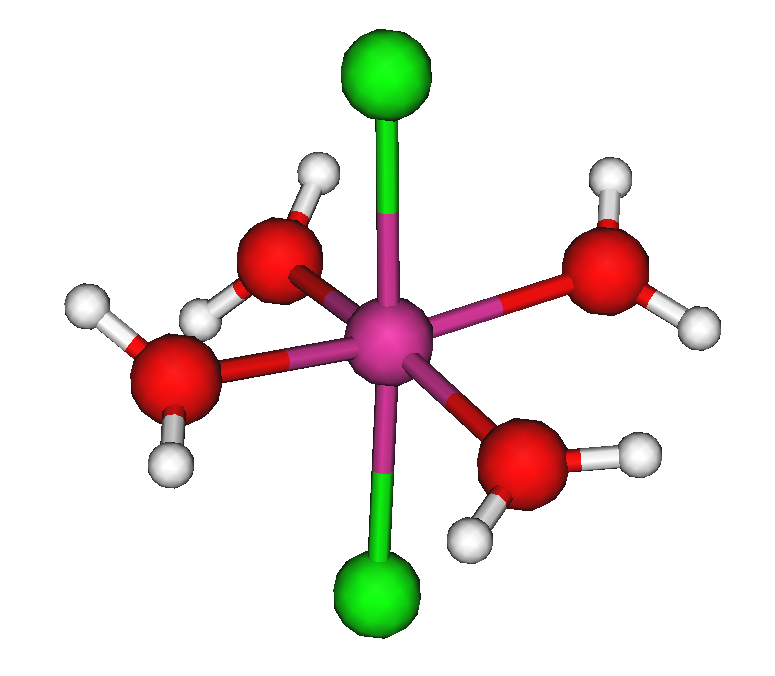
\includegraphics[width=0.2\linewidth]{images/Acuo-trans.png}
			&
			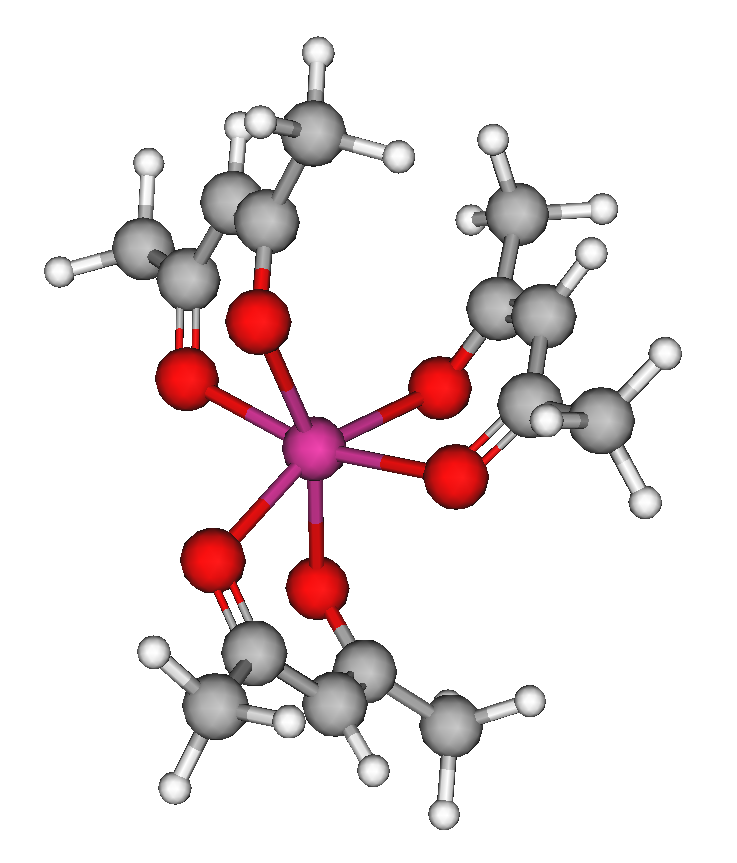
\includegraphics[width=0.2\linewidth]{images/acac-delta.png}
			&
			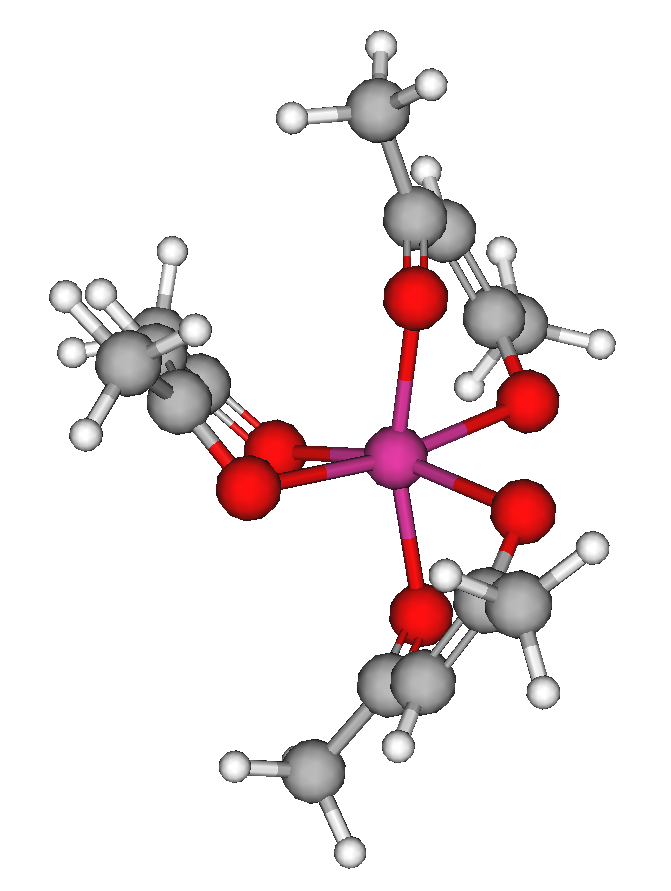
\includegraphics[width=0.2\linewidth]{images/acac-lambda.png}
		\end{tabular}
		\caption{Is\'omeros de los complejos de cromo. A la izquierda los is\'omeros cis-trans del \ce{[CrCl2(H2O)4]+}, a la derecha los is\'omeros $\Delta$-$\Lambda$ \ce{[Cr(acac)3]}.}
		\label{fig: isomeros}
	\end{figure*}
	
	\begin{table}[h]
		\centering
		\caption{Bandas obtenidas para los complejos de cromo.}
		\begin{tabular}{c|cc}
			\multicolumn{1}{l}{} & \ce{[CrCl2(H2O)4]+} & \ce{[Cr(en)3]}  \\
			\hline
			\multirow{2}{*}{$\lambda$ (nm)} & 435.0 & 359.0 \\
			& 625.0 & 470.0  \\
			\hline
			\multirow{2}{*}{Abs (u.a.)}  & 0.156 & 0.346 \\
			& 0.111 & 0.172 \\
			\hline
		\end{tabular}
		\label{tb: resultados}
	\end{table}

	Usando la ley de Lambert–Beer es posible conocer el coeficiente de extinci\'on molar para ambos compuestos:
	\begin{equation}
		\mathcal{E} = \dfrac{A}{cb}
	\end{equation}
	
	Usando la ecuaci\'on anterior y las absorbancias de la \autoref{tb: resultados} se obtiene:
	\begin{table}[h]
		\centering
		\caption{Coeficientes de extinci\'on molar para las dos bandas observadas en los complejos de cromo.}
		\begin{tabular}{c|cc}
			\multicolumn{1}{l}{} & \ce{[CrCl2(H2O)4]+} & \ce{[Cr(en)3]}  \\
			\hline
			\multirow{2}{*}{$\mathcal{E}$ (M$^{-1}$cm$^{-1}$)} & 33.5 & 67.2 \\
			& 23.9 & 32.5 \\
			\hline
		\end{tabular}
		\label{tb: extincion}
	\end{table}
	
	Teniendo en cuenta la energ\'ia de un fot\'on es posible determinar la energ\'ia de un electr\'on para realizar una transici\'on de los de baja energ\'ia del complejo octa\'edrico hasta los de mayor energ\'ia.
	\begin{equation}
		E = h\nu = h\dfrac{c}{\lambda} = \Delta_0
	\end{equation}
	\begin{figure}[h]
		\centering
		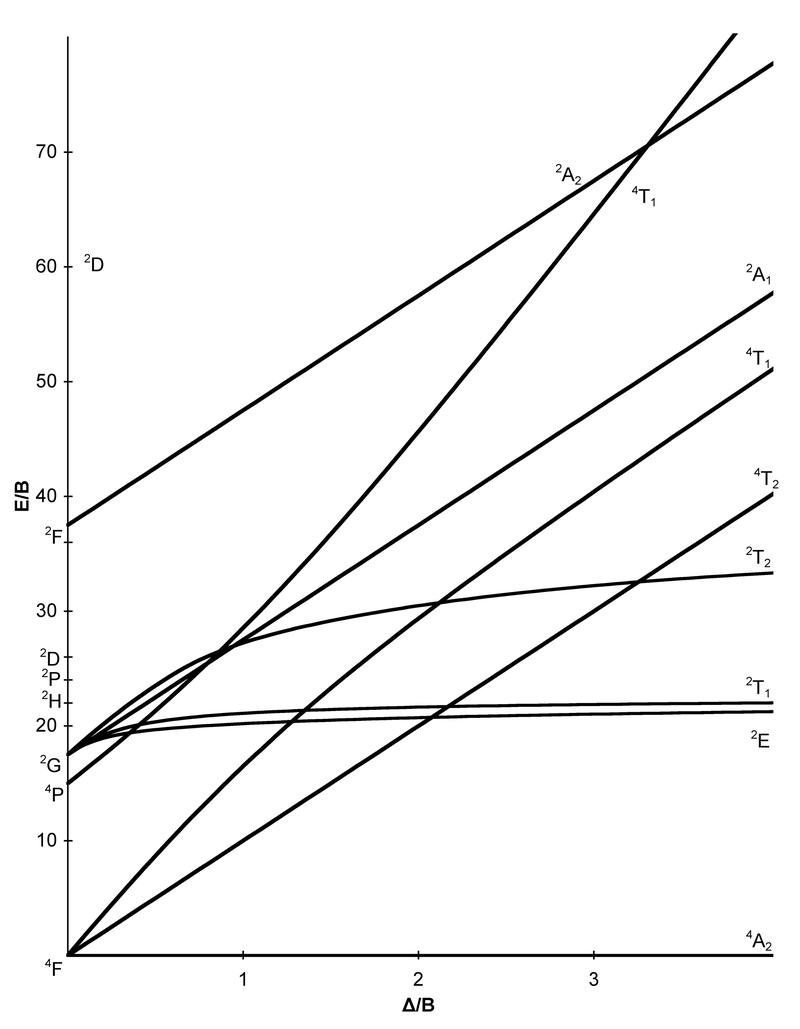
\includegraphics[width=0.9\linewidth]{images/Tanabe-Sugano.png}
		\caption{Diagrama de Tanabe-Sugano para un metal $d^3$.}
		\label{fig: tanabe-sugano}
	\end{figure}
	
	\begin{table}[h]
		\centering
		\caption{Energ\'ia de la transici\'on electr\'onica para los distintos complejos de cromo.}
		\begin{tabular}{c|cc}
			\multicolumn{1}{l}{} & \ce{[CrCl2(H2O)4]+} & \ce{[Cr(en)3]}  \\
			\hline
			\multirow{2}{*}{$E$ (eV)} & 2.85 & 3.45 \\
			& 1.98 & 2.64 \\
			\hline
		\end{tabular}
		\label{tb: energy}
	\end{table}
	
	Con el objetivo de encontrar el par\'ametro de Racah $B$ el cual permite conocer el grado de repulsi\'on entre los electrones enlazados en el complejo, es necesario usar el diagrama de Tanabe-Sugano para un metal $d^3$ el cual se puede observar en la \autoref{fig: tanabe-sugano}. Para $d^3$ el estado basal corresponde con $^4A_{2g}$, dado que se debe mantener el sp\'in las \'unicas transiciones permitidas corresponden con $^4A_{2g} \rightarrow ^4T_{2g}(F)$ y $^4A_{2g} \rightarrow ^4T_{1g}(F)$.
	
	La relaci\'on transici\'on-energ\'ia ($E_2 > E_1$) corresponde con:
	\begin{equation}
		\begin{array}{cc}
			E_1 \implies ^4A_{2g} \rightarrow ^4T_{2g}(F) \\
			E_2 \implies ^4A_{2g} \rightarrow ^4T_{1g}(F)
		\end{array}
	\end{equation}
	
	Con la informaci\'on anterior es posible aplicar un algoritmo con el objetivo de evitar el uso del diagrama de Tanabe-Sugano directamente, dicho algoritmo se encuentra disponible en \href{https://github.com/ricardo-ayres/pynabe-sugano}{\color{blue}GitHub}\footnote{https://github.com/ricardo-ayres/pynabe-sugano}.
	\begin{table}[h]
		\centering
		\caption{Par\'ametros de Tanabe-Sugano.}
		\begin{tabular}{c|cc}
			\multicolumn{1}{l}{} & \ce{[CrCl2(H2O)4]+} & \ce{[Cr(en)3]}  \\
			\hline
			$\Delta_0$ (eV) & 1.98 & 2.63 \\
			$B$ (eV) & 0.089 & 0.077 \\
			\hline
		\end{tabular}
		\label{tb: tanabe}
	\end{table}
	\pagebreak
	
	El resultado de los par\'ametros de Racah para ambos complejos de transici\'on resulta interesante por el orden encontrado. Si bien la etilendiamina es un ligando considerablemente voluminoso, la interacci\'on con el metal tiene lugar con los \'atomos de nitr\'ogeno, los cuales son menos electronegativos que los \'atomos de ox\'igeno y cloro a los que se encuentra coordinado el \ce{[CrCl2(H2O)4]+}, esta diferencia de electronegatividad puede explicar porque la repulsi\'on electroest\'atica es menor para el complejo con etilendiamina.
	
	En el caso de las energ\'ias de estabilizaci\'on tiene sentido el orden encontrado, la etilendiamina es un ligando $\sigma$ donor, lo cual restringe la interacci\'on puesto que no permite retrodonaci\'on. Adem\'as de esto la etilendiamina es un ligando bidentado y considerablemente m\'as voluminoso que los ligandos cloro y acuo. Esto implica que los orbitales $d_{z^2}$ y $d_{x^2-y^2}$ se desestabilizan considerablemente aumentando la energ\'ia del campo cristalino, lo cual a su vez causa una distorci\'on del octa\'edro como se observa en la \autoref{fig: isomeros} con el \ce{[Cr(acac)3]}.
	\section{Preguntas}
	\subsection{El espectro visible del complejo \ce{Cr(acac)_3} es significativamente diferente a los espectros de los otros compuestos, por qu\'e?}
	En la \autoref{fig: isomeros} se observa la diferencia entre los ligando acuo y cloro, respecto al acetilacetonato. El volumen del ligando tiende a distorcionar el octa\'edro generando una mayor degeneraci\'on de los niveles de energ\'ia. Adicionalmente la deslocalizaci\'on de los electrones $\pi$ de los dobles enlaces del carbonil y carbono-carbono permiten la resonancia del acetilacetonato.
	\subsection{El orden de los ligandos obtenido en este experimento corresponde a la serie espectroqu\'imica establecida? Explique cualquier desviaci\'on}
	Como fue discutido en el an\'alisis el orden obtenido fue: $\ce{[Cr(en)3]} > \ce{[CrCl2(H2O)4]+}$, lo cual implica que $\ce{(en)} > \ce{Cl-} \& \ce{H2O}$. 
	
	\subsection{Tomando en cuenta los cambios en los espectros de \ce{CrCl_3 . 6H_2O} durante el tiempo, ?`Cu\'al reacci\'on est\'a ocurriendo?}
	A pesar de no haber obtenido dichos espectros, se puede pensar que la reacci\'on que ocurre es tiene que ver con la sustituci\'on de los ligandos cloro por ox\'igenos, dando lugar a un compuesto binuclear de \'oxido de cromo (III).
	
	\subsection{Bandas d\'ebiles con coeficientes de extinci\'on 1\% son normalmente observados a longitudes de onda grandes en espectros de muchos complejos de Cr (III)}
	Una regla general para la espectroscop\'ia tiene que ver con las intensidades, intensidades bajas implican transiciones prohibidas. En el caso de la espectroscop\'ia UV-vis, las transiciones prohibidas son orbitales $d-d$ y transiciones con cambio de sp\'in. 
	
	\subsection{Mn (II) y Fe (II) son ejemplos para iones de metales de transici\'on que normalmente son m\'as d\'ebilmente coloreados que otros iones de metales de transici\'on.}
	En el caso de los compuestos high sp\'in de estos metales, las coloraciones son d\'ebiles debido a que todas las transiciones son prohibidas por sp\'in.
	
	
	\subsection{Al contrario a la mayor\'ia de los complejos de Mn (II), el compuesto \ce{[Mn(CN)_6]^{4-}} tiene una coloraci\'on muy fuerte.}
	El ligando ciano se encuentra entre los ligandos m\'as fuertes de la serie espectroqu\'imica, esto implica que la energ\'ia de estabilizaci\'on del complejo es considerablemente alta, lo cual da lugar a bandas a longitudes de onda cortas y de alta intensidad.
	
	\section{Conclusiones}	
	A partir del uso del diagrama de Tanabe - Sugano fue posible establecer la energ\'ia de estabilizaci\'on de los dos complejos de coordinaci\'on sintetizados en el laboratorio, adem\'as fue posible explicar el orden obtenido en los par\'ametros de Racah en t\'erminos de las interacciones electroest\'aticas a las que se encuentran sometidos los metales y sus ligandos.
	
	La teor\'ia del campo cristalino permite explicar efectivamente la coloraci\'on de los distintos complejos de coordinaci\'on. La energ\'ia de estabilizaci\'on encontrada para los dos complejos tris(etilendiamin)cromo (III) y tetra(acuo)di(cloro)cromo (III), $\Delta_0 = 2.63$ ,  $\Delta_0 = 1.98$ eV,  concuerda con lo esperado seg\'un la serie espectroqu\'imica. 
	
	\pagebreak
	\phantomsection
	\bibliographystyle{unsrt}
	\begin{thebibliography}{9}
		\bibitem{Orbitals}
		Silberberg, M. S. \textit{Principles of general chemistry}, 2nd ed.; McGraw-Hill: Dubuque, IA, 2009.
		\bibitem{Werner}
		Alfred Werner, (December 12, 1866 - November 15, 1919), Nobel Prize Winner. Retrieved from \textit{Nobelprize.org}.
		\bibitem{Lewis}
		Gilbert Newton Lewis, (October 23, 1875 - March 23, 1946), American physical chemist. Retrieved from \textit{Wikipedia.org}.	
	\end{thebibliography}
\end{document}